\documentclass [10 pt, a4 paper]{article}
\usepackage{booktabs}
\usepackage[utf8]{inputenc}
\usepackage{graphicx}
\usepackage{array}
\usepackage{caption} % for \captionof
\usepackage{amsmath}
\usepackage{verbatim}
\usepackage{listings}
\usepackage{color}
\definecolor{dkgreen}{rgb}{0,0.6,0}
\definecolor{dkblue}{rgb}{0,0,0.6}
\definecolor{mauve}{rgb}{0.58,0,0.82}
\lstset{language=C++,
basicstyle = \ttfamily,
keywordstyle = \color{dkblue},
stringstyle =\color{mauve},
commentstyle = \color{dkgreen},
morecomment=[l][\color{magenta}]{\#}
}
\author{Vincent Richard}
\date{02/11/17}
\title{Computional Method and C++ Assigment}
\setlength\parindent{24pt}

%%%%%%%%%%%%%%%%%%%%%%%%%%%%%%%%%%%%%%%%%%%%%%%%%%%%%%%%%%%%%%%%%%%%%%%%%%%%%%%%%%%%%%%%%%%


\begin{document}

\begin{titlepage}
    \maketitle
\end{titlepage}
\newpage

\tableofcontents
\listoffigures
\newpage

%%%%%%%%%%%%%%%%%%%%%%%%%%%%%%%%%%%    Abstract     %%%%%%%%%%%%%%%%%%%%%%%%%%%%%
\begin{abstract}
    In this assigment we are working on the heat equation, and more precisely on the 
    computation of four schemes in order to find which one of them is the more relevant 
    to use. We are studying two explicits schemes, DuFort-Frankel and Richardson, and two
    implicits schemes, Laasonen and Crank-Nicholson.

    We collected the result of the computation on different time and different time step sizes
    in order to study the error change of each scheme. We found out that the Laasonen scheme is 
    the more accurate. The longer the time is before collecting the result the smaller 
    the error will be. Also there is a linear relation of $f(x) = \frac{1100}{12} x + 18$ 
    between the size of the time step and the error introduce for the Lasonen scheme. So we
    can say regarding our result that Lasonnen is the best choice for calculation with the
    heat equation.
\end{abstract}

%%%%%%%%%%%%%%%%%%%%%%%%%%%%%%%%%    Introduction    %%%%%%%%%%%%%%%%%%%%%%%%%%%%%%%%%%%%%%%%%

\section{Introduction}

In this assignment we are asked to examine the application of numerical schemes
for the solution of partial diferential equations. Compute them and then analyse the accuracy
of everyone of them. In order to  do so we will consider the following probem.

A wall 1 ft. thick and infinite in other directions has an initial uniform temperature Tin of 
100$^{\circ}$F. The surface temperatures Tsur at the two
sides are suddenly increased and maintained at 300$^{\circ}$F. The wall is composed of
nickel steel (40\% Ni) with a diffusivity of D = 0,1 $ft^{2}/hr$.
The governing equation to be solved is the unsteady one-space dimensional
heat conduction equation, which in Cartesian coordinates is:
\begin{equation}
    \frac{\partial T}{\partial t} = D \frac{\partial T}{\partial x^{2}}
\end{equation}

\begin{center}
    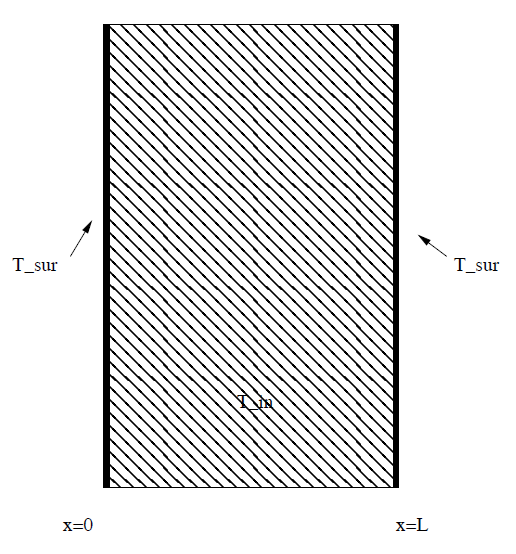
\includegraphics[scale=0.6]{Chart/problem.PNG}
    \captionof{figure}{Representation of the initial problem}
\end{center}

\subsection{Presentation of the different methods used}

\subsubsection{DuFort-Frankel}
The DuFort-Frankel scheme is an explicit scheme unconditionnaly stable of accuracy 
$O((\frac{\Delta t}{\Delta x})^{2}, (\Delta t)^{2},( \Delta x)^{2})$ the parabolic PDE is:
\begin{equation}
    \frac{T_{i}^{n+1} - T_{i}^{n-1}}{2\Delta t} = D \frac{T_{i+1}^{n} -(T_{i}^{n+1} + T_{i}^{n-1}) + T_{i-1}^{n})}{\Delta x^{2}}
\end{equation}
This equation leads to an explicit form which is:
\begin{equation}
    T_{i}^{n+1}(1 + 2r) = T_{i}^{n-1} +2r(T_{i+1}^{n} - T_{i}^{n-1} + T_{i-1}^{n}), r =\frac{D\Delta t}{\Delta x^{2}}
\end{equation}

\subsubsection{Richardson}
The Richardson scheme is an explixit scheme, unconditionnaly unstable of accuracy $O((\Delta t)^{2},( \Delta x)^{2})$:
\begin{equation}
    \frac{T_{i}^{n+1} - T_{i}^{n-1}}{2\Delta t} = D \frac{T_{i+1}^{n} - 2 T_{i}^{n} + T_{i-1}^{n}}{\Delta x^{2}}
\end{equation}
This equation leads to an explicit form which is:
\begin{equation}
    T_{i}^{n+1} = 2r(T_{i+1}^{n} - 2T_{i}^{n} + T_{i-1}^{n}) + T_{i}^{n-1}, r=\frac{D\Delta t}{\Delta x^{2}}
\end{equation}

\subsubsection{Laasonen}
The Laasonen scheme is an implicit scheme unconditionnaly stable of accuracy $O(\Delta t, (\Delta x)^{2})$,
that as for equation:
\begin{equation}
    \frac{T_{i}^{n+1} - T_{i}^{n-1}}{2\Delta t} = D\frac{T_{i+1}^{n} - 2T_{i}^{n} + T_{i-1}^{n}}{\Delta x^{2}}
\end{equation}

This equation leads to a form that result in a system of linear equation:
\begin{equation}
    -r T_{i+1}^{n+1} + (1+2r)T_{i}^{n+1} -rT_{i-1}^{n+1} =T_{i}^{n}, r=\frac{D\Delta t}{\Delta x^{2}}
\end{equation}

\subsubsection{Cranck-Nicholson}
The Crank-Nicholson scheme is an implicit scheme unconditionnaly stable of accuracy $O((\Delta t)^{2}, (\Delta x)^{2})$, that as for equation:
\begin{equation} 
    \frac{T_{i}^{n+1} - T_{i}^{n}}{\Delta t} = \frac{D}{2}(\frac{T_{i+1}^{n+1}-2T_{i}^{n+1}+T_{i-1}^{n+1}}{\Delta x^{2}} + \frac{T_{i+1}^{n}-2T_{i}^{n}+T_{i-1}^{n}}{\Delta x^{2}})
\end{equation}

This equation leads to a form that result in a system of linear equation:
\begin{equation}
    -\frac{r}{2} T_{i+1}^{n+1}+(1+r)T_{i}^{n+1}-\frac{r}{2}T_{i-1}^{n+1} = \frac{r}{2}T_{i+1}^{n} + (1-r)T_{i}^{n} + \frac{r}{2}T_{i-1}^{n}
\end{equation}
\quad

\newpage

%%%%%%%%%%%%%%%%%%%%%%%%%%%%%     Methods Procedures      %%%%%%%%%%%%%%%%%%%%%%%%%%%%%%%%%%%%%

\section{Methods and Procedures}

\subsection{Code Structure}

    To resolve the problem we decided to create an oriented object program base on 
those figures (for readibility reason I divided the structure in three graphics):
\begin{center}
    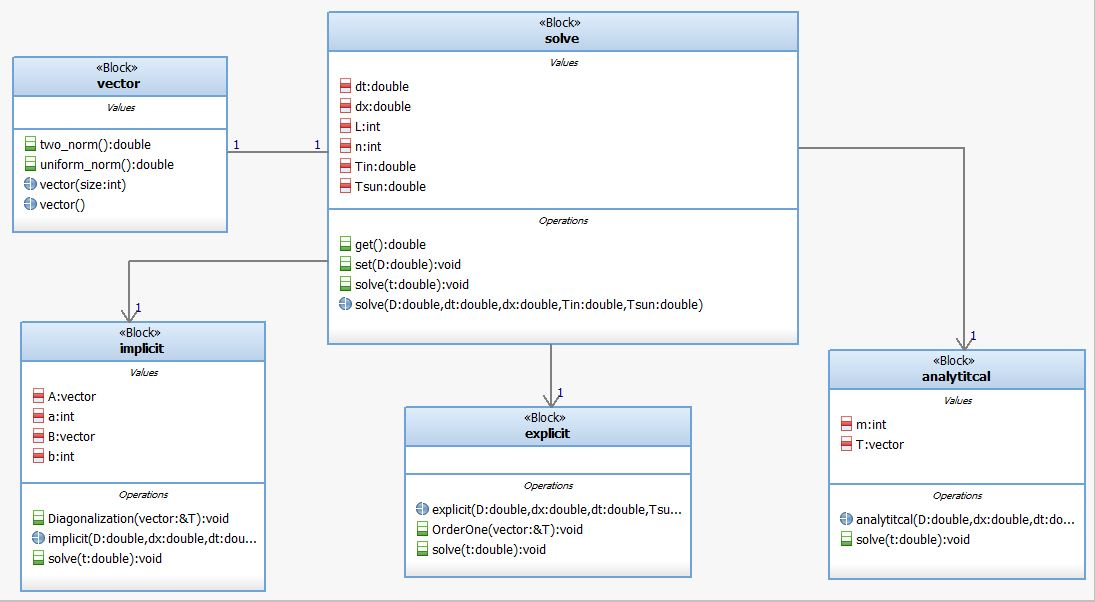
\includegraphics[scale=0.6]{Chart/General.JPG}
    \captionof{figure}{General Architecture}
\end{center}
%%%%%%%%%%%%% Solve
The based class is \textbf{Solve}. It has a number of argument:
\begin{itemize}
    \item D the diffusivity which is in the assigment of $D = 0.1$  \textit{$ft^{2}$/hr}
    \item dt the gap in time between n and n+1
    \item dx the gap in space between i and i+1
    \item Tin the initial temperature of the wall here $Tin = 100^{\circ}F$
    \item Tsun the temperature on the two sides that are maintained at $Tsun = 300^{\circ}F$
    \item L the lenght of the wall which is fix to 1 ft. in this exercice
    \item n the number of possible position x for a fixed t, it calculated with $n = \frac{L}{dx}$
\end{itemize}

\vspace{0.3cm}
It also has couples of methods:
\begin{itemize}
    \item Solve(double D, double dx, double dt, double Tsun, double Tin), the only constructor of 
    this class and initialize the different value depending on the user input
    \item solve(double t) a virtual method that is created to be use in the derived class it will be the function
    that solve and print the result of the problem
    \item get() / set() methods, basic accessor methods
\end{itemize}

\vspace{0.3cm}
The \textbf{Solve} class also have three derived class \textbf{Implicit}, \textbf{Explicit}, and \textbf{Analytical}.
The \textbf{Implicit} and \textbf{Explicit} class are further details below. We now will talk about the \textbf{Analytical} class.
%%%%%%%%%%%%%%%% Analytical
\vspace{0.3cm}

The class \textbf{Analytical} calculate the analytical solution of the input problem.
The class provided two new arguments:
\begin{itemize}
    \item m is an integer used to simplify the expression of T since the anatical value of T is : 
    \begin{equation}
        T = T_{sur} + 2(T_{in}-T_{sur}) \sum_{m=1}^{m=\infty} e^{-D(m\pi /L)^{2}t} \frac{1-(-1)^{m}}{m\pi} sin(\frac{m\pi x}{L})
    \end{equation}

    We need to get a smaller m for the upper border of the sum. We choosed to fix it at 10 000, 
    the result obtain was an approximation under 0.5\% so we decided it was accurate enough to do 
    the simplification.

    \item T is a vector defined as an argument to to be able to call it from the main program
\end{itemize}
The \textbf{Analytical} class has also two methods:
\begin{itemize}
    \item The constructor Analytical(...), is based on the constructor of the solve class, it also
    initialize the value of m and the vector T
    \item The solve function that is here defined to print the value of the analytical solution T 
    of the problem with the approximation as explain above. It will print the value of T at each $10dt$hr
    until the argument t is reach
\end{itemize}

%%%%%%%%%%%%%%%% Vector
\vspace{0.3cm}

The \textbf{Vector} class is associated with the \textbf{Solve} class, it is use to defined 
vector in the derived class.
The methods of the vector class:
\begin{itemize}
    \item one\_norm
    \item two\_norm
    \item uniform\_norm
\end{itemize}
are used to calculate each type of vector norm and will be of use to calculate the accuracy of each scheme.

%%%%%%%%%%%%%% Explicit
\begin{center}
    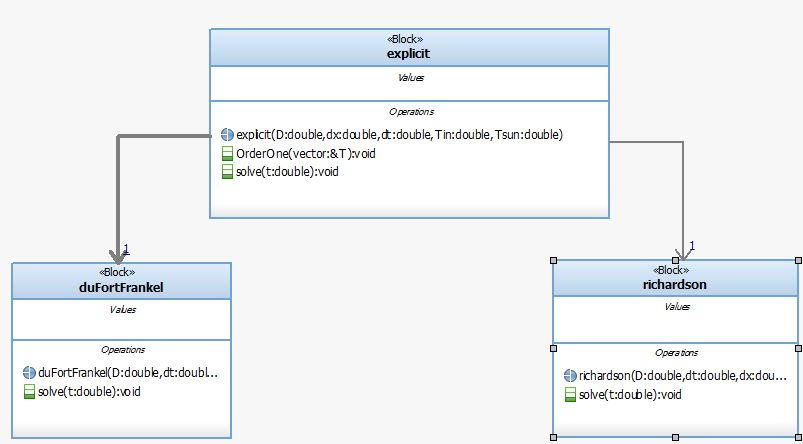
\includegraphics[scale=0.6]{Chart/Explicit.JPG}
    \captionof{figure}{Explicit Architecture}
\end{center}

The derived \textbf{Explicit} class is also a based class for two other class: the \textbf{DuFortFrankel}
class and the \textbf{Richardson} class. Each of them solving the problem with the scheme of the same name.

\vspace{0.3cm}

The \textbf{Explicit} class define 3 new arguments:
\begin{itemize}
    \item Tpast, T, and Tnext are vector declared in the explicit class because they will be used
    in both derived class. It is also to be able to use their values from the main class.
\end{itemize}

The \textbf{Explicit} class has the same methods as the \textbf{Solving}class. But it does define an aditionnal method. 

The \textbf{OrderOne} method was created because in the two explicit schemes, DuFort-Frankel
and Richardson, we encounter the issue of not being able to start the scheme at $n = 1$.
To find the value of the temperature T at a time n we need the value of T at n and n-1 (See equation (3) and (5)).
The problem set the values of T at $n = 0$ but we still need to find T at $n=1$ to use those
schemes. So we first need the method \textbf{OrderOne} to find T at $n = 1$ with a forward time central
space scheme, and then apply the Richardson and DuFort-Frankel scheme to find the other values 
of T.

Since this method is useful for both derived class, we decided to declare it in the 
\textbf{Explicit} class.


The two derived classes \textbf{DuFortFrankel} and \textbf{Richardson} work the same way.

They have the same constructor method based on the one defined in the \textbf{Explicit} class
and they both defined the method \textbf{solve} in a very similar way. 

Once the initialisation of T at $n = 1$ (with the \textbf{OrderOne} method) 
is done, we use a loop, depending on the scheme, the equation (3) or (5) will be use to
iterate the values of T until we reach the value of t wanted by the user.
%%%%%%%%%%%%%%%%% Implicit

\begin{center} 
    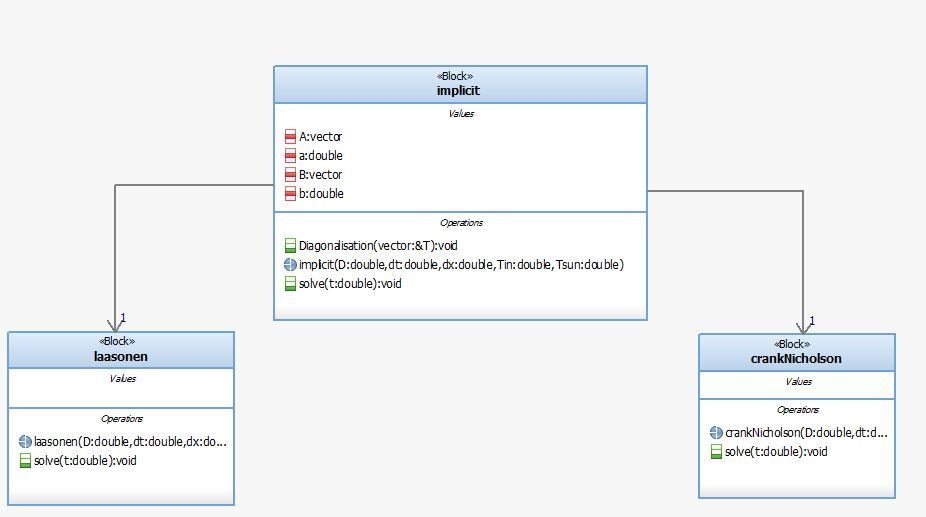
\includegraphics[scale=0.6]{Chart/Implicit.JPG}
    \captionof{figure}{Implicit Architecture}
\end{center}

The derived \textbf{Implicit} class is also a based class for two other classes: the 
\textbf{Laasonen} class and the \textbf{Cranck-Nicholson} class. Each of them solving 
the problem with the scheme of the same name.

The \textbf{Implicit} class just like the \textbf{Explicit} as a particular method to 
simplify the solving of the problem in the two derived classes as well as two new defined vector Tpast and Tnext.
To understand what the \textbf{Diagonalization} method is used for we need to talk about
the resolution of the problem for the two implicit schemes.

\vspace{0.3cm}

The two system of equation that we wrote in equation (7) and (8) can be written like this:

\begin{equation}
\begin{pmatrix} b    &    a   &    0   & \cdots &   0    \\
a    & \ddots & \ddots & \ddots & \vdots \\
0    & \ddots & \ddots & \ddots &    0   \\
\vdots & \ddots & \ddots & \ddots &   a    \\ 
0    & \cdots &    0   &   a    &    b   \\
\end{pmatrix}
=
\begin{pmatrix} T_{0}^{n+1} \\ 
\vdots \\ 
T_{imax}^{n+1} \\
\end{pmatrix}
R
\end{equation}
Where a, b are doubles and R a vector, all of their values change depending on 
which scheme we choose. Since the problem is a tri-diagonal matrix and for each scheme,
we have (in the special case of the data given by the assigment) 
$ 2\left \| a \right \| \leq \left \| b \right \| $ so we can use Thomas algorithm to
solve those equation.

Thomas Algorithm is an efficient way of solving tridiagonal matrix systems. It is based
on LU decompositionin which the matrix system $Mx = r$ is rewritten as $LUx = r$ where L 
is a lower triangular matrix and U is an upper triangular matrix. The system can be 
efficiently solved by setting $Ux = p$ and then solving first $Lp = r$ for p and then 
$Ux=p$ for x. The Thomas algorithm consist of two steps. In step one decomposing the matrix
into $M=LU$ and solving $Lp=r$ are accomplished in a single downwards sweep, taking us
straight from $Mx=r$ to $Ux=p$. In step two the equation $Ux=p$ is solved for x in  an
upward sweep.

In the \textbf{Diagonalization} we are taking care of the first step of the Thomas algorithm.
We will have this kind of equation at the end of the method:

\begin{equation}
\begin{pmatrix} 1    &    B_{0}    & \cdots &   0    \\
                0    & \ddots     & \ddots  & \vdots \\
                \vdots & \ddots & \ddots & B_{imax - 1}  \\ 
                0    & \cdots   &   0    &    1   \\
\end{pmatrix}
=
\begin{pmatrix} T_{0}^{n+1} \\ 
\vdots \\ 
T_{imax}^{n+1} \\
\end{pmatrix}
P
\end{equation}
The values of $B_{i}$ and P will be stored respectively in the B vector and the A
vector defined in the \textbf{Implicit} class.

The function \textbf{solve} in both \textbf{Cranck-Nicholson} and \textbf{Laasonen} 
is a loop that initialize the vector R (with the help of the equation (7) and (9),
call the method \textbf{Diagonalization(R)} and then calculate the second step of the
Thomas algorithm. It will print for each $10dt$hr the value of T until the time t in the
argument of solve is reached.
\vspace{0.5cm}

To run this program we use a \textbf{main.cpp} file that will create an object in each file
and depending the input of the user (note that the user can change only the values of the measuring time t
and the step size dt) it will call the function wanted.

We also add a function \textbf{accuracy} that will calculate the absolute and relative error of the scheme needed
only at the measuring time needed.

We will now see the data collecting procedure.

%%%%%%%%%%%%%%%%%%%%%%%%%%%%%%%%%%%%%%        Data Gathering        %%%%%%%%%%%%%%%%%%%%%%%%

\subsection{Data Gathering}

In this Assigment there is different type of Data that we are looking for.
First of all we want to find all the values of the different scheme for each 0.1hr until 0.5hr.
In order to find this data we use the \textbf{solve} method explained before, that will print 
the values of T every $10dt$ until the input time t is reach. So we use as step time size 
dt = 0.01hr and t = 0.5hr in each scheme to find the Data we need.

Furthermore we want to find the accuracy of each method. To collect this data we defined a function
\textbf{accuracy}, it will use the value of T for each scheme, this value is the one calculate for
the input t, so the T at the end of the each \textbf{solve} method. 
We based the calculation of this function on the absolute error and the relative error.
Their equation are respectively:
\begin{equation}
    AE = \left \| T_{scheme} - T_{ana} \right \|, RE = \frac{\left \| T_{scheme} - T_{ana} \right \|}{\left \| T_{scheme} \right \|}
\end{equation}

Since we are in a one base problem we will use the l1-norm that as the following definition:

\begin{equation}
    \left \| x \right \|_{1} = \sum_{i} \left \| x_{i} \right \|
\end{equation}

As for the required compution time, we try to implement a timer in the laasonen \textbf{solve} method
but even in nanoseconds it keeped printing bolean values. So we haven't been able to collect proper data
for this part.
%%%%%%%%%%%%%%%%%%%%%%%%%%%%%%%%%%%%%%            RESULT             %%%%%%%%%%%%%%%%%%%%%%%
\newpage
\section{Result}
\subsection{Comparasion with the Analytical result}

Those graphics are the result given by the program with $dt = 0.01hr$ and $dx = 0.05ft$, 
we printed for each scheme the curve of t = 0.1ht to t = 0.5hr: 

\begin{center} 
    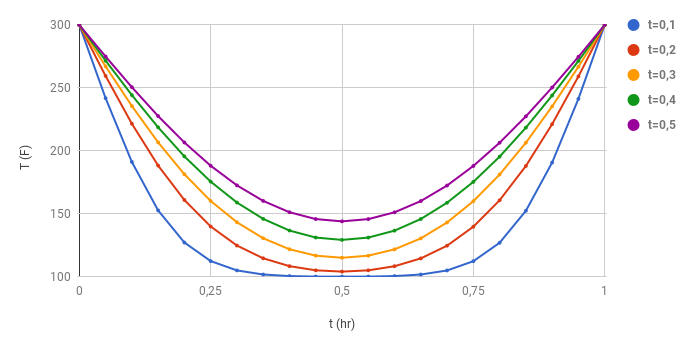
\includegraphics[scale=0.5]{Chart/analytical.PNG}
    \captionof{figure}{Analytical Result}
\end{center}

\begin{center} 
    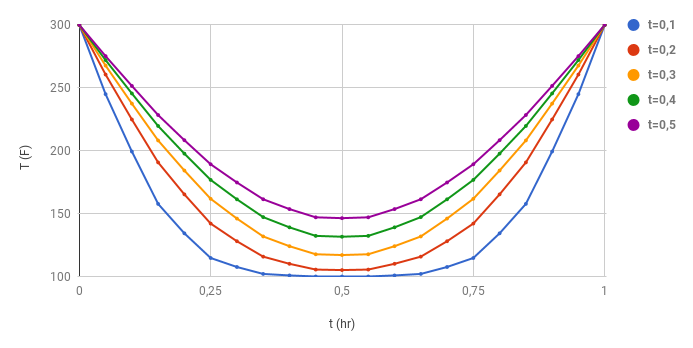
\includegraphics[scale=0.5]{Chart/duFortFrankel.PNG}
    \captionof{figure}{DuFort-Frankel Result}
\end{center}

\begin{center} 
    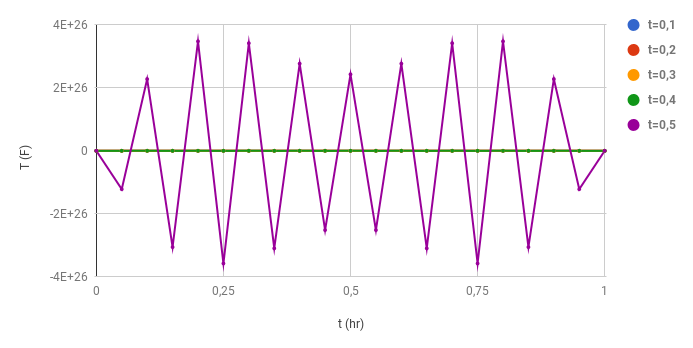
\includegraphics[scale=0.5]{Chart/richardson.PNG}
    \captionof{figure}{Richardson Result}
\end{center}

\begin{center} 
    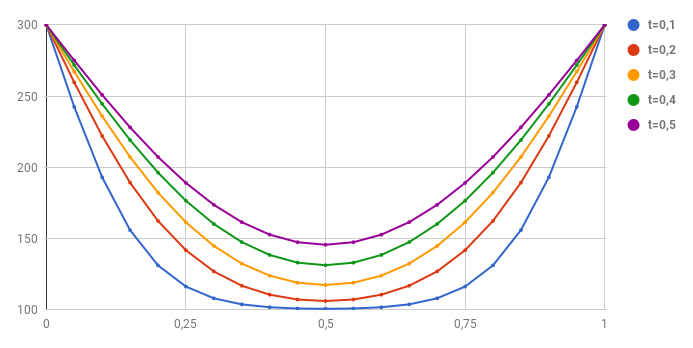
\includegraphics[scale=0.5]{Chart/laasonen.PNG}
    \captionof{figure}{Laasonen Result}
\end{center}

\begin{center} 
    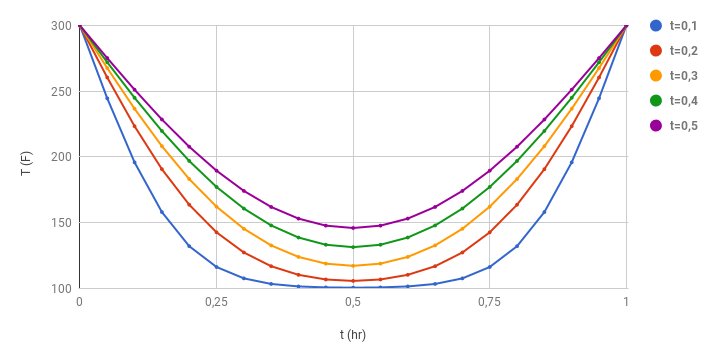
\includegraphics[scale=0.5]{Chart/crankNicholson.PNG}
    \captionof{figure}{Cranck-Nicholson Result}
\end{center}
 
We can conclude that all the scheme except \textbf{Richardson} are stable.
It was predictable since Richardson was the only scheme that was unconditionnaly
unstable. The other scheme are all unconditionnaly stable and very similar to the Analytical
result, it is hard to see which one is the more accurate.

To find out we have calculated the absolute and relative Error (with a fixed $dt = 0.01hr$), we get those graphics:

\begin{center} 
    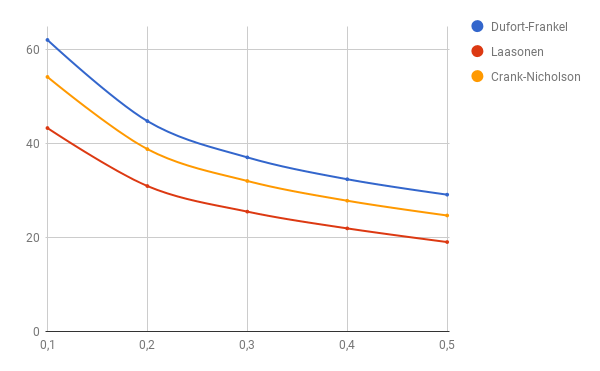
\includegraphics[scale=0.5]{Chart/AbsoluteError.PNG}
    \captionof{figure}{Absolute Error Calculation}
\end{center}

\begin{center} 
    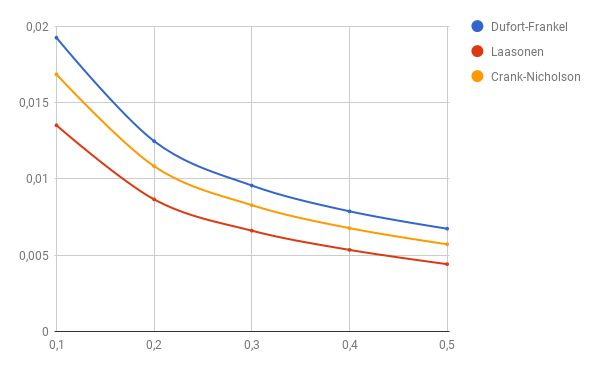
\includegraphics[scale=0.5]{Chart/RelativeError.PNG}
    \captionof{figure}{Relative Error Calculation}
\end{center}

Those graphics shows that all three schemes get more accurate as the time grows higher.
We may be able to explain that the first value are highly inacurate by the fact that the analytical 
solution is an approximation and even if this one is close to the actual answer it still includes 
additional error in the result we get with the shemes.

In all cases it is clear that the Laasonen scheme is more accurate than the other since all schemes have
the same behaviour and that the initial value of the lasonnen error scheme is smaller. 
But we can also notice that all of the schemes are pretty accurate since at $t = 0.3 hr$ all 
of them have an error below 1\%. We can predict that the error will continue to get smaller until 
it reach 0. All schemes tend to reach 0, because they are exposed to the continuous surface temperature. 
To show this behaviour we try to find the error at t=10hrs, we get :

DuFort Frankel Absolute Error: 0.00695182,  Relative Error: 1.103e-006

Laasonen Absolute Error: 0.00797042, Relative Error: 1.265e-006

Crank-Nicholson Absolute Error: 0.000457142, Relative Error: 7.256e-008
\vspace{0.1cm}

The error is now much more smaller and it is now Cranck-Nicholson that is the more accurate scheme.
It doesn't mean that Crank-Nicholson is more suitable for calculation, because once t = 10 hr is reach the
values are all around 0 and we can't get data out of it.
So this seconf result is not very intersting, except that it proves that all scheme will reach 0 when t tend 
to infinity.

\newpage
\subsection{Laasonen study}
We will now study the effect of the step size on the accuracy on the Laasonen scheme.
Once we retrieve all the data we get for an input t = 0.5hr:

\begin{center} 
    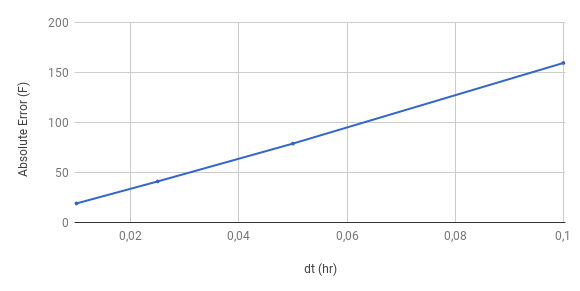
\includegraphics[scale=0.5]{Chart/laasonenAE.PNG}
    \captionof{figure}{Absolute Error of the Laasonen scheme plotted against the step size}
\end{center}

We can observe that the increasing of the step size has a direct effect on the error, the bigger
the step size will be the less accurate the scheme will become. Furthermore it seems that 
there is a linear relationship between those two variables. We can calculate an approximation of this
equation: 

$f(x) = \frac{1100}{12} x + 18$.

As for the study of the computtional time, I wasn't able to implement a working timer so I can't
show any result for this question. But since the number of loop to compute to a certain time depend on the
value of the step size, we can guess that as the step size increased, the computation time decrease.

%%%%%%%%%%%%%%%%%%%%%%%%%%%%%%%%%%%%%        CONCLUSION      %%%%%%%%%%%%%%%%%%%%%%%%%%%%%%%%%%%%%%%%
\section{Conclusion}
Based on the result we have we can say that the Laasonen scheme has the best accuracy and so that
it is more suitable to do calculation. Depending on our need we will have to choose between a total accurate
result and a faster program. But since the Laasonen scheme reach a an error $<1\%$ in less than 0.2hr
It is possible to have a good balance in both parameters.



%%%%%%%%%%%%%%%%%%%%%%%%%%%%%%%%%%%%%%          References                   %%%%%%%%%%%%%%%%%%%%%%%%%%%%%%%%%
\section{References}
\begin{enumerate}
    \item http://www.industrial-maths.com
    \item http://www.math.pku.edu.cn
    \item Von Newmann Stability Analysis, Dr.Johnson 2008
\end{enumerate}

%%%%%%%%%%%%%%%%%%%%%%%%%%%%%%%%       APPENDICE        %%%%%%%%%%%%%%%%%%%%%%%%%%%%%%%%%%%%%%%%%
\section{Appendice}
\subsection{Richardson Analysis}
We are gonna study the Richardson scheme accuracy and Stability. In this Assigment we used this expression
to calculate Richardson:
\begin{equation}
    \frac{T_{i}^{n+1} - T_{i}^{n-1}}{2\Delta t} - D \frac{T_{i+1}^{n} - 2 T_{i}^{n} + T_{i-1}^{n}}{\Delta x^{2}} = 0
\end{equation}

To find the accuracy of this scheme we are going to rewrite some term with the Fourrier expansion:

\begin{equation}
    T_{i}^{n+1} = T_{i}^{n} + (\frac{\partial T}{\partial t})_{i}^{n} \Delta t + (\frac{\partial^{2} T}{\partial t^{2}})_{i}^{n} \frac{\Delta t^{2}}{2!} + O(\Delta t^{3})
\end{equation}

\begin{equation}
    T_{i}^{n-1} = T_{i}^{n} - (\frac{\partial T}{\partial t})_{i}^{n} \Delta t + (\frac{\partial^{2} T}{\partial t^{2}})_{i}^{n} \frac{\Delta t^{2}}{2!} + O(\Delta t^{3})     
\end{equation}

\begin{equation}
    T_{i+1}^{n} = T_{i}^{n} + (\frac{\partial T}{\partial x})_{i}^{n} \Delta x + (\frac{\partial^{2} T}{\partial x^{2}})_{i}^{n} \frac{\Delta x^{2}}{2!} + (\frac{\partial^{3} T}{\partial x^{3}})_{i}^{n} \frac{\Delta x^{3}}{3!} + O(\Delta x^{4})     
\end{equation}

\begin{equation}
    T_{i-1}^{n} = T_{i}^{n} - (\frac{\partial T}{\partial x})_{i}^{n} \Delta x + (\frac{\partial^{2} T}{\partial x^{2}})_{i}^{n} \frac{\Delta x^{2}}{2!} - (\frac{\partial^{3} T}{\partial x^{3}})_{i}^{n} \frac{\Delta x^{3}}{3!} O(\Delta x^{4})         
\end{equation}

We then implement those equations in the first Richardson equation, we get:

\begin{equation}
    (\frac{\partial T}{\partial t})_{i}^{n} - D (\frac{\partial^{2} T}{\partial x^{2}})_{i}^{n} + O(\Delta t^{2}, \Delta x^{2}) = 0
\end{equation}

We can see that we recovered the initial equation. So T is the solution of the continuous error,
but also the solution of the discreted problem with some error which is included in $O(\Delta t^{2}, \Delta x^{2})$.
The accuracy of the Richardson scheme is $O(\Delta t^{2}, \Delta x^{2})$.

We will now study the stability of this scheme, to do so we will do a Von Newmann Stability Analysis:
A numerical scheme is said to be stable if deviation from exact solution decreases in time.
So we need to de compose the residual error.

If we consider T the solution of the ortignal problem and $\tau$ the solution of the discreted probem
we will have:

$T_{i}^{n} = \tau_{i}^{n} + r_{i}^{n}$

So we have:
\begin{equation}
    r_{i}^{n+1} - r_{i}^{n-1} = 2\alpha (r_{i+1}^{n} - 2 r_{i}^{n} + r_{i-1}^{n}), \alpha = \frac{D \Delta t}{\Delta x^{2}}
\end{equation}
We decompose the error: 
\begin{equation}
    r_{i}^{n} = \sum_{-\infty }^{+\infty } g^{n}(k) e^{ikx_{i}} 
\end{equation}

and get the following equation after considering it for only one wave:

$g^{n+1}e^{ikx_{i}} - g^{n-1}e^{ikx_{i}} = 2\alpha(g^{n}e^{ikx_{i+1}} -2 g^{n}e{ikx_{i} + g^{n}e^{ikx_{i-1}}})$

$g^{n-1}e^{ikx_{i}}(g^{2} - 1) = 2\alpha g^{n}e^{ikx_{i}}(e^{ik\Delta x} - 2 + e^{-ik\Delta x})$

$g^{2} - 1 = 2\alpha g (2cos(k \Delta x) -2)$, because $2cos(\theta) = e^{i\theta} + e^{-i\theta} $

$g^{2} - 1 = -6\alpha g sin^{2}(\frac{k\Delta x}{2})$, because $ 2sin^{2}(x) = 1 - cos(2x)$

So we finaly get: 
$g^{2} + 6\alpha g sin^{2}(\frac{k\Delta x}{2}) - 1 = 0$

This quadratic equation has two roots, the sum and the product of the two roots are given by:

$g_{1} + g_{2} = - 6 \alpha sin^{2}(\frac{k\Delta x}{2})$, and $g_{1} g_{2} = -1$

For the scheme to be stable we need $\left \|  g_{1} \right \| \leq 1$ and $\left \|  g_{2} \right \| \leq 1$.
The product of the roots show that if $\left \|  g_{1} \right \| < 1$ then $\left \|  g_{2} \right \| > 1$
and vice-versa. Also if $g_{1} = 1$ and $g_{2} = -1$ then we must have $\alpha = 0$.

We can conclude that the Richardson scheme is unconditionnaly unstable.

\subsection{Code}
You will find in this part all my code:


 
This is my \texttt{main.cpp}:
\lstinputlisting{../main.cpp}

This is my \texttt{solve.cpp}:
\lstinputlisting{../Class/Solver/solve.cpp}

his is my \texttt{solve.h}:
\lstinputlisting{../Class/Solver/solve.h}

This is my \texttt{vector.cpp}:
\lstinputlisting{../Class/Useclass/vector.cpp}

This is my \texttt{analytical.cpp}:
\lstinputlisting{../Class/Solver/Analytical/analytical.cpp}

This is my \texttt{analytical.h}:
\lstinputlisting{../Class/Solver/Analytical/analytical.h}

This is my \texttt{explicit.cpp}:
\lstinputlisting{../Class/Solver/Explicit/explicit.cpp}

This is my \texttt{explicit.h}:
\lstinputlisting{../Class/Solver/Explicit/explicit.h}

This is my \texttt{implicit.cpp}:
\lstinputlisting{../Class/Solver/Implicit/implicit.cpp}

This is my \texttt{implicit.h}:
\lstinputlisting{../Class/Solver/Implicit/implicit.h}

This is my \texttt{duFortFrankel.cpp}:
\lstinputlisting{../Class/Solver/Explicit/DuFort-Frankel/duFortFrankel.cpp}

This is my \texttt{duFortFrankel.h}:
\lstinputlisting{../Class/Solver/Explicit/DuFort-Frankel/duFortFrankel.h}

This is my \texttt{richardson.cpp}:
\lstinputlisting{../Class/Solver/Explicit/Richardson/richardson.cpp}

This is my \texttt{richardson.h}:
\lstinputlisting{../Class/Solver/Explicit/Richardson/richardson.h}

This is my \texttt{laasonen.cpp}:
\lstinputlisting{../Class/Solver/Implicit/Laasonen/laasonen.cpp}

This is my \texttt{laasonen.h}:
\lstinputlisting{../Class/Solver/Implicit/Laasonen/laasonen.h}

This is my \texttt{crankNicholson.cpp}:
\lstinputlisting{../Class/Solver/Implicit/Crank-Nicholson/crankNicholson.cpp}

This is my \texttt{crankNicholson.h}:
\lstinputlisting{../Class/Solver/Implicit/Crank-Nicholson/crankNicholson.h}

\end{document}